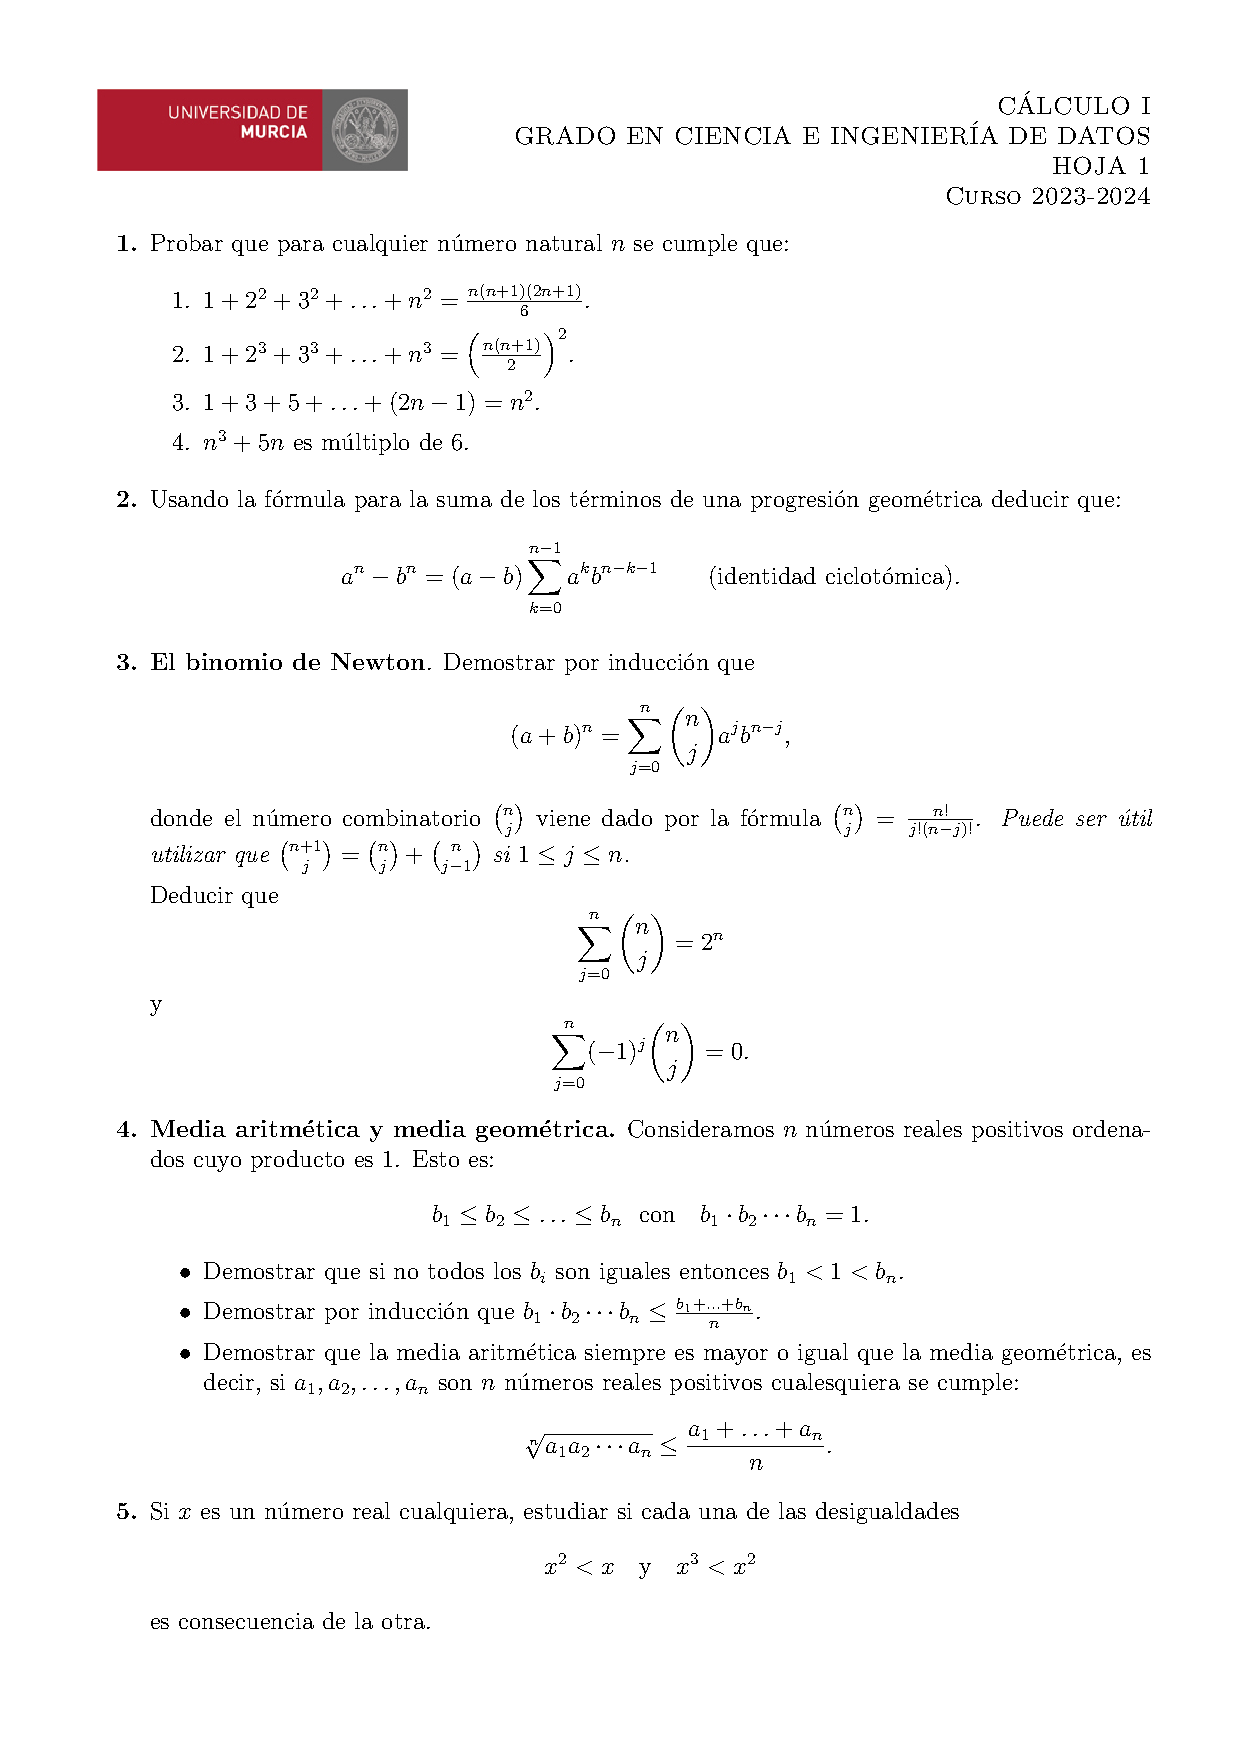
\includepdf[page=-]{Tema 1/Hoja 1 Murcia/Hoja 1 Murcia.pdf}

\begin{enumerate}[label=\color{red}\textbf{\arabic*)}, leftmargin=*]
	\item \textcolor{lightblue}{Probar que para cualquier número natural $n$ se cumple que:}
	\begin{enumerate}[label=\color{red}\arabic*)]
		\item \textcolor{blue}{$1+2^2+3^2+\cdots+n^2=\dfrac{n(n+1)(2n+1)}{6}$}
		\item \textcolor{blue}{$1+2^3+3^3+\cdots+n^3=\left(\dfrac{n(n+1)}{2}\right)^2$}
		\item \textcolor{blue}{$1+3+5+\cdots+(2n-1)=n^2$}
		\item \textcolor{blue}{$n^3+5n$ es un múltiplo de 6}
	\end{enumerate}
	\item \textcolor{lightblue}{Usando la fórmula para la suma de los términos de una progresión geométrica deducir que: \[ a^n-b^n=(a-b)\sum_{k=0}^{n-1}a^kb^{n-k-1}\qquad\text{(identidad ciclotómica)}. \]}
	
	\item \textcolor{lightblue}{\textbf{El binomio de Newton.} Demostrar por inducción que \[ (a+b)^n=\sum_{j=0}^{n}\binom{n}{j}a^jb^{n-j} \] donde el número combinatorio $\binom{n}{j}$ viene dado por la fórmula $\binom{n}{j}=\dfrac{n!}{j !(n-j)!}$. \textit{Puede ser útil utilizar que $\mathit{\binom{n+1}{j}=\binom{n}{j}+\binom{n}{j-1}}$ si $\mathit{1\le j\le n}$}.\\
	Deducir que \[ \sum_{j=0}^{n}\binom{n}{j}=2^n \] y \[ \sum_{j=0}^{n}(-1)^{j}\binom{n}{j}=0. \]}
	\item \textcolor{lightblue}{\textbf{Media aritmética y media geométrica.} Consideremos $n$ números positivos ordenados cuyo producto es 1. Esto es: \[ b_1\ge b_2\ge\dots\ge b_n\quad\text{con}\quad b_1\cdot b_2\cdots b_n=1 \]}
	\begin{itemize}[label=\color{red}\textbullet]
		\item \db{Demostrar que si no todos los $b_i$ son iguales entonces $b_1<1<b_n$.}
		\item \db{Demostrar por inducción que $b_1\cdot b_2\cdots b_n\le\dfrac{b_1+\cdots+\b_n=1}{n}$.}
		\item \db{Demostrar que la media aritmética siempre es mayor o igual que la media geométrica, es decir, si $a_1,a_2,\dots,a_n$ son $n$ números reales positivos cualesquiera se cumple: \[ \sqrt[n]{a_1a_2\cdots a_n}\le\dfrac{a_1+\cdots+a_n}{n}. \]}
	\end{itemize}
	\item \textcolor{lightblue}{Si $x$ es un número real cualquiera, estudiar si cada una de las desigualdades \[ x^2<x\quad\mathrm{y}\quad x^3<x^2\] es consecuencia de la otra.}
	
	\[ \begin{aligned}
		x^2<x & \longleftrightarrow  x^2-x<0\\
		 & \longleftrightarrow x(x-1)<0\\
		 & \longleftrightarrow x\in(0,1)\\
		 & \longrightarrow x<1\\
		 & \longrightarrow x^3<x^2 
	\end{aligned} \]
	La implicación en sentido contrario no es cierta. Para $x=-1,~~-1=x^3<x^2=1$, sin embargo, $x^2=1$ no es menor que $x=-1$.
	\item \textcolor{lightblue}{Sea $0<a<1$, demostrar que la sucesión $z_n=a(a^{2n}+(-1)^n)$ no tiene límite.}
	
	Basta con tomar la subsucesión de términos pares, es decir, $z_{2n}=a(a^{4n}+1)\longrightarrow a$, mientras que la subsucesión de términos impares, $z_{2n+1}=a(a^{2n+1}-1)\longrightarrow-a$. Por lo que el límite no existe, dado que en caso de existe toda subsucesión convergente a dicho límite.
	\item \textcolor{lightblue}{Sea $(x_n)_n$ una sucesión de números reales convergente. Supongamos que los términos de la sucesión son alternativamente positivos y negativos. Calcular su límite.}
	
	En este caso, el límite es igual a 0. Supongamos que el límite $l>0$, entonces, utilizando la definición de convergencia, tendríamos que para $\epsilon\coloneq l>0$ existe un $n_0\in\mathbb{N}$ tal que si $n\ge n_0$ entonces \begin{equation}\label{ecuación}
		|x_n-l|<\epsilon=l.
	\end{equation} Puesto que los términos son alternativamente positivos y negativos, podemos afirmar que existe $n_1>n_0$ tal que $n_{n_1}<0$, luego \[ |x_{n_1}-l|=l-x_{n_1}>l=\epsilon, \] lo cual es una contradicción con la desigualdad (\ref{ecuación}) , luego no es cierto que $l>0$. De igual forma se puede razonar que $l$ no puede ser negativo, siendo, por tanto, el límite $l=0$.
	\item \textcolor{lightblue}{Sea $(t_n)_n$ una sucesión que verifica $0\le t_n\le 1~\forall n\in\mathbb{N}$. Sean $(x_n)_n$ e $(y_n)_n$ dos sucesiones convergentes al número $z$. Probar que la sucesión \[ (t_nx_n+(1-t_n)y_n)_n, \] también converge al número $z$.}
	
	Puesto que $(x_n)_n$ es convergente a $z$. Para $\epsilon>0$ existe $n_1\in\mathbb{N}$ tal que si $n\ge n_1$ entonces \[ |x_n-z|<\epsilon. \]
	De igual forma, para $(y_n)_n$ convergente a $z$, existe $n_2\in\mathbb{N}$ tal que si $n\ge n_2$ entonces \[ |y_n-z|<\epsilon. \]
	Fijado $\epsilon$, \[ \begin{aligned}
		|t_nx_N+(1-t_n)y_n-z|&=|t_nx_n+(1-t_n)y_n-z-\cancel{t_nz}+\cancel{t_nz}|\\
		&=|t_n(x_n-z)+(1-t_n)(y_n-z)|\\
		&\le|t_n|\cdot|x_n-z|+|1-t_n|\cdot|y_n-z|\\
		&=t_n\cdot|x_n-z|+(1-t-n)\cdot|y_n-z|
	\end{aligned} \]
	Ahora si $n\ge n^*\coloneq\max\{n_1,n_2\}$ tenemos que la expresión anterior verificará que \[ \le t_n\cdot\epsilon+(1-t_n)\cdot\epsilon=\epsilon. \]
	Luego para cada $\epsilon>0$ podemos encontrar un número natural, $n^*$ tal que si $n\ge n^*$ entonces \[ |t_nx_n+(1-t_n)y_n-z|<\epsilon, \] es decir, la sucesión converge a $z$.
	\item \textcolor{lightblue}{Sea $A$ un conjunto no vacío de números reales. Si $A$ está acotado superiormente, describir una sucesión de elementos de $A$ convergente hacia el supremos de $A$.}
	
	Sea $\alpha\coloneq\sup\{A\}$. Entonces para cada $n\in\mathbb{N}$, tenemos que $\alpha-\dfrac{1}{n}$ no es el supremo de $A$, por lo cual existirá un elemento $a_n\in A$ tal que \[ \alpha-\dfrac{1}{n}\le a_n\le \alpha. \] De esta forma construimos una sucesión $(a_n)$, que por el teorema de bocadillo tendrá como límite $\alpha$.
	\item \textcolor{lightblue}{Sea $(x_n)_n$ una sucesión de números reales positivos y sea $\beta=\lim_{n\to\infty}\dfrac{x_{n+1}}{x_n}$.}
	\begin{enumerate}[label=\color{red}\arabic*)]
		\item \textcolor{blue}{Si $\beta<1$ entonces $(x_n)_n$ converge a cero.}
		
			Puesto que $\beta=\lim_{n\to\infty}\dfrac{x_{n+1}}{x_n}$ entonces fijado $\epsilon>0$ existe $n_0\in\mathbb{N}$ tal que si $n\ge n_0$ entonces \[ \left|\dfrac{x_{n+1}}{x_n}-\beta\right| <\epsilon\] es decir, \[ |x_{n+1}-\beta x_n|<\epsilon\cdot|x_n| \] y aquí, puesto que $x_n>0$ para cada $n\in\mathbb{N}$. \[ |x_{n+1}-\beta x_n|<\epsilon\cdot x_n. \]
		Ahora, \[ \begin{array}{c}
			-\epsilon\cdot x_n<x_{n+1}-\beta\cdot x_n<\epsilon\cdot x_n\\
			(\beta-\epsilon)\cdot x_n<x_{n+1}<(\beta+\epsilon)\cdot x_n.
		\end{array} \] Recordaremos que la desigualdad anterior es cierta para cada $n\ge n_0$ y observamos que \[ (\beta-\epsilon)\cdot x_{n+1}<x_{n+2}<(\beta+\epsilon)\cdot x_{n+1} \] Pero a su vez tenemos \[ (\beta-\epsilon)^2x_n<(\beta-\epsilon)\cdot x_{n+1}<x_{n+2}<(\beta+\epsilon)\cdot x_{n+1}<(\beta+\epsilon)^2x_n, \] es decir, para cada $m\in \mathbb{N}$  \begin{equation}\label{ec2}
			(\beta-\epsilon)^mx_n<x_{n+m}<(\beta+\epsilon)^mx_n. 
		\end{equation}
		Si $0<\beta<1$, podemos tomar $\epsilon>0$ tal que $0<\beta-\epsilon<\beta+\epsilon<1$. Luego $(x_n)$ se encuentra acotada entre dos sucesiones convergentes a 0, luego su límite es 0.
		\item \textcolor{blue}{Si $\beta>1$ entonces $(x_n)_n$ diverge a $+\infty$.}
		
			Si $\beta>1$, entonces podemos encontrar $\epsilon>0$ tal que $\beta-\epsilon>0$ y la desigualdad (\ref{ec2}) obtenemos que para cada $m\in\mathbb{N}$, \[ (\beta-\epsilon)^mx_n<x_{n+m}, \] y $(\beta-\epsilon)^mx_n$ converge a $\infty$ cuando $m\to\infty$, luego lo mismo le sucede a la sucesión $(x_{n+m})_{m}$, y de aquí a la sucesión $(x_n)_n$.
		\item \textcolor{blue}{Mostrar mediante dos ejemplos que si $\beta=1$ no podemos asegurar nada.}
		
			Si $\beta=1$ no podemos asegurar nada. Ejemplo: $x_n=\dfrac{1}{n}$. El límite $\lim_{n\to\infty}\dfrac{\frac{1}{n+1}}{\frac{1}{n}}=\lim_{n\to\infty}\dfrac{n}{n+1}=1$. El límite de la sucesión $(x_n)_n=\left(\dfrac{1}{n}\right)_n$ es 0. Por otra parte si tomamos la sucesión $y_n=n$, vemos que el valor de $\beta$ obtenido es 1 y la sucesión $y_n$ es divergente.
		\item \textcolor{blue}{Calcular el límite de las sucesiones $x_n=\dfrac{10^n}{n!}=\dfrac{n!}{(2n+1)!}$.}
		Por último, vamos a utilizar este criterio para determinar el límite de las sucesiones que nos indican. 
		$x_n=\dfrac{10^n}{n!}>0$ \[ \lim_{n\to\infty}\dfrac{\frac{10^{n+1}}{(n+1)!}}{\frac{10^n}{n!}}=\lim_{n\to\infty}\dfrac{10}{n+1}=0<1 \] Luego la sucesión $(x_n)_n$ tiene límite igual a 0.
		
		$y_n=\dfrac{n!}{(2n+1)!}$ \[ \lim_{n\to\infty}\dfrac{\frac{(n+1)!}{(2n+3)!}}{\frac{n!}{(2n+1)!}}=\lim_{n\to\infty}\dfrac{n+1}{(2n+3)(2n+2)}=0<1 \] Luego el límite de la sucesión $(y_n)_n$ es igual a 0.
	\end{enumerate}
	\item \textcolor{lightblue}{Probar que la sucesión $(x_n)_{n\ge1}$ dada por: \[ x_n=\sum_{k=1}^{n}\dfrac{1}{n+k}=\dfrac{1}{n+1}+\dfrac{1}{n+2}+\cdots+\dfrac{1}{n+n} \] es creciente y está acotada superiormente.}
	\[ x_{n+1}=\sum_{k=1}^{n+1}\dfrac{1}{n+1+k}=\sum_{k=2}^{n+2}\dfrac{1}{n+k}. \] Ahora \[ \begin{aligned}
		x_{n+1}-x_n&=\sum_{k=2}^{n}\dfrac{1}{n+k}+\dfrac{1}{2n+1}+\dfrac{1}{2n+2}-\dfrac{1}{n+1}-\sum_{k=2}^{n}\dfrac{1}{n+k}\\
		&=\dfrac{1}{2n+1}+\dfrac{1}{2(n+1)}-\dfrac{1}{n+1}\\
		&=\dfrac{1}{2n+1}-\dfrac{1}{2n-2}\\
		&>0,
	\end{aligned} \] luego $x_{n+1}>x_n$ para cada $n\in\mathbb{N}$. Para demostrar que está acotada superiormente basta con observar que \[ x_N=\sum_{k=1}^{n}\dfrac{1}{n+k}=\dfrac{1}{n+1}+\dfrac{1}{n+2}+\cdots+\dfrac{1}{n+n}\le\dfrac{n}{n+1}=1-\dfrac{1}{n+1}, \] es decir, $(x_n)_n$ está acotada por una sucesión que es convergente (y por tanto está acotado).
	\item \lb{Sea $x_1=1$. Definimos por recurrencia:}
	\begin{enumerate}[label=\color{red}\alph*)]
		\item $\db{x_{n+1}=\dfrac{x_n}{4}}$
		\item $\db{x_{n+1}=\dfrac{x_n}{n+1}}$
		\item $\db{x_{n+1}=\dfrac{n}{n+1}x_n}$
		\item $\db{x_{n+1}=1+\dfrac{x_n}{2}}$
	\end{enumerate}
	\lb{Probar que, cada una de ellas, es monótona y acotada. Hallar sus límites.}
	\item \lb{Sea $(x_n)_{n\ge1}$ una sucesión de números que cumple \[ x_{n+1}=\sqrt{2x_n}\quad\text{para}\quad n\in\mathbb{N}. \] Determinar para qué valores de $x_1\ge0$ la sucesión es convergente y calcular su límite en cada caso.}
	\item \lb{Sea $(x_n)_{n\ge1}$ una sucesión de números reales que cumple \[ x_{n+1}\dfrac{x_n^2+2}{2x_n} \] y $x_1>0$. Comprobar que $(x_n)_{n\ge1}$ es decreciente (a partir del segundo término en algunos casos), que está acotada inferiormente por $\sqrt{2}$ y que tiene límite $\ell=\sqrt{2}$.}
	\item \lb{Sea $(x_n)_n$ la sucesión definida por la relación de recurrencia: $7x_{n+1}=x_n^3+6\quad n=1,2,\dots$ Demostrar que si $x_1=\dfrac{1}{2}$ entonces la sucesión es convergente y calcular su límite. ¿Qué ocurre si $x_1=\dfrac{3}{2}$?}
	
	Observamos que $x_{n+1}=\dfrac{1}{7}x_n^3+\dfrac{6}{7}$. Demostramos por inducción que la sucesión es monótona creciente. Efectivamente, $x_2=\dfrac{7}{8}>x_1=\dfrac{1}{2}$. Además podemos afirmar que $x_n\ge0$ para cada $n\in\mathbb{N}$. Supongamos que $x_n\ge x_{n-1}$. De aquí, $x_{n+1}=\dfrac{x_n^3+6}{7}\le\dfrac{x_{n-1}^3+6}{7}=x_n$. Por otra parte tenemos que la desigualdad $x_{n+1}\ge x_n$ se cumple si y sólo si $x^3-7x_n+6\ge0$, es decir, $(x_n-1)(x_n-2)(x_n+3)\ge0$. Desigualdad, ésta última, que se cumple cuando $x_n\in[-3,1]\cup[2,+\infty)$. Vamos a demostrar por inducción que la sucesión está acotada por 1. Trivialmente, $x_1=\dfrac{1}{2}\le1$. Si $x_n\le1$ entonces \[ x_{n+1}=\dfrac{x_n^3+6}{7}\le\dfrac{1^3+6}{7}=1, \] por lo que la acotación está demostrada. Por último, podemos que el límite de la sucesión será 1. Basta con tomar límites en ambos términos de la expresión $x_{n+1}=\dfrac{x_n^3+6}{7}$ para obtener que la única solución posible es 1.
	
	Si $x_1=\dfrac{3}{2}$, veremos que en este caso la sucesión es decreciente. \[ x_2=\dfrac{75}{56}<\dfrac{3}{2}. \] Si $x_n\le x_{n-1}$ entonces $x_{n+1}=\dfrac{x_n^3+6}{7}\le\dfrac{x_{n-1}^3+6}{7}=x_n$. Ahora siguiendo con razonamiento similar podemos demostrar que $x_n\ge1$ para cada $n\in\mathbb{N}$. $x_1\le1$. Supongamos que $x_n\ge1$ entonces $x_{n+1}=\dfrac{x_n^3+6}{7}\ge\dfrac{1+6}{7}=1$. De nuevo concluimos que la sucesión es convergente y que el límite es igual a 1. 
	\item \lb{Se define por recurrencia $a_1=2,\quad a_{n+1}=\dfrac{2a_n}{a_n+3},n\in\mathbb{N}$.}
	\begin{enumerate}[label=\color{red}\roman*)]
		\item \db{Demostrar que la sucesión $(a_n)_n$ converge.}
		\item \db{Hallar el límite de $(a_n)_n$.}
		\item \db{Sea el subconjunto de números reales dado por $A=\{a_1,a_2,\dots,a_n,\dots\}$. Determinar justificadamente si existe supremo, ínfimo, máximo y mínimo de $A$ y dar, en su caso, los valores de los mismos.}
	\end{enumerate}
	
	Veamos que la sucesión es decreciente. Observa además que $a_n>0,a_1>0$ y $a_{n+1}=\dfrac{2a_n}{a_n+3}>0$ si $a_n>0$, para cada $n\in\mathbb{N}$. Ahora \[ \dfrac{a_{n+1}}{a_n}=\dfrac{1}{a_n+3}\le\dfrac{2}{3}<1, \] es decir, $a_{n+1}\le a_n$ para cada $n\in\mathbb{N}$. Ahora el límite $l$ debe cumplir que \[ \begin{array}{c}
		l=\dfrac{2l}{l+3},\\
		l(l+1)=0.
	\end{array} \]De donde obtenemos que el límite de la sucesión es igual a 0 puesto que $a_n>0$ para cada $n\in\mathbb{N}$.
	
	Ahora, el supremo y el máximo coinciden con el valor 2. El ínfimo es igual a 0. El conjunto $A$ no tienen mínimo.
	\item \lb{Se define por recurrencia $a_1=9,a_{n+1}=\sqrt{a_n}+2$. Decidir justificadamente si la sucesión $\{a_n\}$ es convergente. En caso afirmativo, calcular su límite.}
	
	La sucesión es decreciente. $a_2=5$. Por inducción, supongamos que $a_n\le a_{n-1}$, de aquí, $a_{n+1}=\sqrt{a_n}+2\le\sqrt{a_{n-1}}+2=a_n$. Veamos ahora que $a_n\ge3$ para $n\in\mathbb{N}$. Lo hacemos por inducción, supongamos $a_n\ge4$, entonces $a_{n+1}=\sqrt{a_n}+2\ge\sqrt{4}+2=4$
	\item \lb{Sea $(x_n)_n$ la sucesión definida por la relación de recurrencia: $x_{n+1}=x_n+\dfrac{1}{x_n}\quad n=1,2,\dots$ ¿Es convergente la sucesión si $x_1=x>0$?}
	\item \lb{Sean $a,b\in\mathbb{R}$ tales que $0<a<b$. Se definen la sucesiones $(a_n)_n,(b_n)_n\subset\mathbb{R}$ por recurrencia como: $a_1=a, b_1=b$ y \[ a_{n+1}=\sqrt{a_nb_n}\quad\text{y}\quad b_{n+1}=\dfrac{a_n+b_n}{2}. \]}
	\begin{enumerate}[label=\color{red}\roman*)]
		\item \db{Probar que las sucesiones son convergentes.}
		\item \db{Probar que convergente al mismo número}
	\end{enumerate}
	\item \lb{Sea $(x_n)_n$ una sucesión verificando: $|x_n|\le2$ y $|x_{n+2}-x_{n+}|\le\dfrac{1}{8}|x_{n+1}^2-x_n^2|\:\forall\,n\in\mathbb{N}$. Demostrar que la sucesión es convergente.}
	
	\[ \left|x_{n+2}-x_{n+1}\right| \le\dfrac{1}{8}\left|x_{n+1}-x_n\right|\cdot\left|x_{n+1}+x_n\right|\le\dfrac{1}{8}\left|x_{n+1}-x_n\right|\cdot\left(\left|x_{n+1}\right|+\left|x_n\right|\right)\le\dfrac{1}{2}\left|x_{n+1}-x_{n}\right|\] Por tanto, \[ \begin{array}{c}
		|x_2-x_1|\le\dfrac{1}{2}|x_1-x_0|\\
		|x_3-x_2|\le\dfrac{1}{2^2}|x_1-x_0|\\
		|x_4-x_3|\le\dfrac{1}{2^3}|x_1-x_0|\\
		\cdots\\
		|x_{n+1}-x_n|\le\dfrac{1}{2^n}|x_1-x_0|\\
		\begin{aligned}
			|x_{n+m}-x_n|&\le|x_{n+m}-x_{n+m-1}|+|x_{n+m-1}-x_{n+m-2}|+\cdots+\left|x_{n+2}-x_{n-1}\right|+\left|x_{n+1}-x_n\right|\\
			&\le\left(\dfrac{1}{2^{n+m-1}}+\dfrac{1}{2^{n+m-2}}+\cdots+\dfrac{1}{2^{n+1}}+\dfrac{1}{2^n}\right)|x_1-x_0|\\
			&=\dfrac{\frac{1}{2^n}-\frac{1}{2^{n+m}}}{\frac{1}{2}}|x_1-x_0|\\
			&=\dfrac{1}{2^{n-1}}\cdot\left(1-\dfrac{1}{2^m}\right)|x_1-x_0|
		\end{aligned}
	\end{array} \] Luego la sucesión es de Cauchy y por tanto es convergente.
	\item \lb{Sea $(x_n)_{n\ge1}$ una sucesión de números reales definida por: \[ x_n=\sqrt{n+\sqrt{(n-1)+\cdots+\sqrt{2+\sqrt{1}}}}. \]}
	\begin{enumerate}[label=\color{red}\arabic*)]
		\item \db{Demostrar que para cada número natural $n\in\mathbb{N}$ se verifica que: \[ \sqrt{n}\le x_n\le2\sqrt{n}. \]}
		\item \db{Probar que la sucesión \[ \left(\dfrac{x_n}{\sqrt{n}}\right)_{n\ge1} \] converge hacia 1.}
		\item \db{Determinar el límite de $(x_n-\sqrt{n})_{n\ge1}$}
		\end{enumerate}	
		Observamos que $x_n=\sqrt{n+x_{n-1}}$, siendo $x_1=\sqrt{1}=1$. Además $x_n>0$ para cada $n\in\mathbb{N}$. $n<n-x_{n-1}$, luego $\sqrt{n}<\sqrt{n+x_{n-1}}=x_n$. Para demostrar la otra desigualdad procedemos a utilziar inducción	para demostrar que $x_n\le2\sqrt{n}$. Efectivamnete, $x_1=\sqrt{1}\le2\cdot1=2$. Supongamos que $x_n\le2\sqrt{n}$ entonces $x_{n+1}=\sqrt{n+1+x_n}\le\sqrt{n+1+2\sqrt{n}}$. Ahora, 
		\begin{align*}
			\sqrt{n+1+2\sqrt{n}}\le2\sqrt{n+1}&\Longleftrightarrow n+1+2\sqrt{n}\le4(n+1)\\
			&\Longleftrightarrow 2\sqrt{n}\le3(n+1)\\
			&\Longleftrightarrow2\sqrt{n}\le3(n+1)\\
			&\Longleftrightarrow4n\le9(n^2+1+2n)\\
			&\Longleftrightarrow0\le9n^2+14n+9
		\end{align*}
		Esta última desigualdad es cierta para cada $n\in\mathbb{N}$. Recordar que todos los valores considerados en las desigualdades no pueden ser negativos.
		
		Una vez que tenemos la desigualdad dividiendo por $\sqrt{n}$ obtenemos \[ 1\le\dfrac{x_n}{\sqrt{n}}\le2, \]es decir, es una sucesión acotada.
		
		Observamos que \[ \dfrac{x_n}{\sqrt{n}}=\dfrac{\sqrt{n+x_{n-1}}}{\sqrt{n}}=\sqrt{1+\dfrac{x_{n-1}}{n}} \] pero \[ \sqrt{n-1}\le x_{n-1}\le2\sqrt{n-1}, \] y de aquí \[ \dfrac{1}{\sqrt{n}}\cdot\sqrt{1-\dfrac{1}{n}}\le\dfrac{x_{n-1}}{n}\le\dfrac{2}{\sqrt{n}}\cdot\sqrt{1-\dfrac{1}{n}}. \]
		De donde, \[ \sqrt{1+\dfrac{1}{\sqrt{n}}\cdot\sqrt{1-\dfrac{1}{n}}}\le\dfrac{x_n}{\sqrt{n}}\le\sqrt{1+\dfrac{2}{\sqrt{n}}\cdot\sqrt{1-\dfrac{1}{n}}} .\] Por el teorema del bocadillo tenemos que el límite existe y es igual a 1.
		
		Por último veamos que \[ \lim_{n\to\infty}x_n-\sqrt{n}=\dfrac{1}{2}. \] Efectivamente, \begin{align*}
			\lim_{n\to\infty}x_n-\sqrt{n}&=\lim_{n\to\infty}\sqrt{n+x_{n-1}}-\sqrt{n}\\
			&=\lim_{n\to\infty}\sqrt{n}\cdot\left(\sqrt{1+\dfrac{x_{n-1}}{n}}-1\right)\\
			&=\lim_{n\to\infty}\sqrt{n}\cdot\left(\sqrt{1+\dfrac{x_{n-1}}{\sqrt{n-1}}\cdot\dfrac{\sqrt{n-1}}{n}}-1\right)\\
			&=\lim_{n\to\infty}\sqrt{n}\cdot\dfrac{1}{2}\cdot\dfrac{x_{n-1}}{\sqrt{n-1}}\cdot\dfrac{\sqrt{n-1}}{n}\\
			&=\dfrac{1}{2}.
		\end{align*}
	\item \lb{Si $(x_n)_n$ es de Cauchy, demostrar que entonces se cumple: \[ \forall\,\epsilon>0\exists\,n_0\in\mathbb{N}:|x_{n+1}-x_n|<\epsilon\:\forall\,n\ge n_0. \] Comprobar con la sucesión $(\sqrt{n})_n$ que esta condición no es suficiente para que una sucesión sea de Cauchy.}
	
		Fijado $\epsilon>0$ para $n\ge n_0$ tenemos que \[ |x_{m+n}-x_n|\le\epsilon \] En particualr para $m=1$ obtenemos el resultado buscado\\
	La sucesión $(\sqrt{n})$ es divergetne, por tanto no es de Cauchy, sin embargo, \[ \sqrt{n+1}-\sqrt{n}=\sqrt{n}\cdot\left(\left(1+\dfrac{1}{n}\right)^{\frac{1}{2}}-1\right)\equiv\sqrt{n}\cdot\dfrac{1}{2}\cdot\dfrac{1}{n}\longrightarrow0.\]
	\item \lb{\textit{Sucesiones Contractivas}. Sea $(x_n)_{n\ge1}$ una sucesión de números reales para el que existe un número real $K\in[0,1)$ y tal que, oara cada número natural $n\ge2$, se tiene que: \[ \left|x_{n+1}-x_n\right| \le K\left|x_n-x_{n-1}\right|.\] Demostrar que la sucesión $(x_n)_{n\ge1}$ es de Cauchy.}
	
	\[ \begin{array}{c}
		|x_3-x_2|\le K|x_2-x_1|\\
		|x_4-x_3|\le K^2|x_2-x_1|\\
		|x_5-x_4|\le K^3|x_2-x_1|\\
		\\
		|x_{n+1}-x_n|\le K^3|x_2-x_1|\\
		\begin{aligned}
			|x_{n+m}-x_n|&\le|x_{n+m}-x_{n+m-1}|+|x_{n+m-1}-x_{n+m-2}|+\left|x_{n+m-2}-x_{n`m-3}\right|+\cdots+\left|x_{n+2}-x_{n+1}\right|+\left|x_{n+1}-x_n\right|\\
			&\le\left(K^{n+m-1}+K^{n+m-2}+K^{n+m-3}+\cdots+K^n\right)\left|x_2-x_1\right|\\
			&=\dfrac{K^n-K^{n+m}}{1-K}\left|x_2-x_1\right|
		\end{aligned}
	\end{array} \]
	Puesto que $K\in[0,1)$ podemos encontrar $n_0\in\mathbb{N}$ tal que $\dfrac{K^n-K^{n+m}}{1-K}|x_2-x_1|<\epsilon$ para $n\ge n_0$.
	\item \begin{enumerate}[label=\color{red}\arabic*)]
		\item \lb{Calcular el límite de $x_n=\sum_{k=1}^{n}\dfrac{1}{k(k+1)}$.}
		
		\[ \dfrac{1}{k(k+1)}=\dfrac{A}{k}+\dfrac{B}{k+1}, \] de donde $A=1$ y $B=-1$. \[ S_n=\sum_{k=1}^{n}\dfrac{1}{k(k+1)}=\sum_{k=1}^{n}\dfrac{1}{k}-\dfrac{1}{k+1}=1-\dfrac{1}{n+1}\xrightarrow[n\to\infty]{}1 \]
		\item \lb{Probar que toda sucesión $(x_n)_n$ que cumple: $\left|x_{n+1}-x_n\right|<\dfrac{1}{n(n+1)}\forall\,n\in\mathbb{N}$ es de Cauchy.}
		Al igual que hemos razonado en el ejercicio anterior tenemos que \[ \left|x_{n+m}-x_n\right| \le\sum_{k=1}^{m}\left|x_{n+k}-x_{n+k-1}\right|\le\sum_{k=1}^{m}\dfrac{1}{n(n+1)},\]que es convergente.
		\item \lb{Demostrar que $x_n=\sum_{k=1}^{n}\dfrac{\sin(kx)}{k(k+1)}$ es convergente.}
		
		Observa que $\left|x_{n+1}-x_n\right|=\left|\dfrac{\sin((n+1)x)}{(n+1)(n+2)}\right|\le\dfrac{1}{(n+1)(n+2)}$ y por el apartado anterior es de Cauchy, y por tanto, convergente.
\end{enumerate}
\item \lb{Si la sucesión $(n_k)_{k\ge1}$ es estrictamente creciente, entonces para cada $k\in\mathbb{N}$, se tiene que $n_k\ge k$.}

Dada $k\in\mathbb{N}$ existirá un $n\in\mathbb{N}$ tal que $n\ge k$. Sea $\{k\in\mathbb{N}:n_k\le k\}$. Este elemento tendrá un máximo $n_{k_0}$, luego $n_{k_0+1}$ no pertenecerá al conjunto y verificará la condición que $k<n_{k_0+1}$.
\item \lb{En las siguientes afirmaciones, decir cuales son verdaderas y cuales son falsas. Probar las que sean verdaderas y proporcionar un contraejemplo para las que sean falsas.}
\begin{enumerate}[label=\color{red}\alph*)]
	\item \db{Toda sucesión acotada que tiene una subsucesión convergente, es convergente.}
	
	Falso. Ejemplo: $x_n=(-1)^n$
	\item \db{Toda sucesión monótona crecietne que tiene una subsucesión convergente, es convergente.}
	
	Verdadero.
	
	Supongamos que $(x_{nk})_k$ es convergente a $l$. Entonces para cada $\epsilon>0$ existe $k_0\in\mathbb{N}$ que si $k\ge k_0$ entonces $\left|x_{n_k}-l\right|=l-x_{n_k}<\epsilon$. Ahora si $n\ge n_k$ entonces $x_n\ge x_{n_{k_0}}$ puesto que es creciente. Ahora \[ \left|x_n-l\right| =l-x_n\le l-x_{n_{k_0}}<\epsilon.\]
\end{enumerate}
\item \lb{Sea $(x_n)_n$ una sucesión de números reales. Probar que se verifca el siguiente resultado: $(x_n)_n$ es convergetne su y sólo si $(x_{2n})_n$ y $(x_{2n-1})_n$ son convergentes y con el mismo límite.}

Observamos que si $(x_n)_n$ es convergente cualquier subsucesión es convergetne al mismo límite, en particular, las dos subsucesiones que se nos indican. Por otra parte, supongamos que ambas subsucesiones que se nos indican. Por otra parte, supongamos que ambas subsucesiones son convergentes al mismo límite. Entonces para cada $\epsilon>0$ existe $n_0\in\mathbb{N}$ tal que si $n\ge n_0$ entonces \[ \left|x_{2n}-l\right| <\epsilon\] y \[ \left|x_{2n-1}-l\right|<\epsilon. \] Luego $(x_n)$ converge a $l$.
\item \lb{Sea $(x_n)_n$ una sucesión de números reales que verifica que las subsucesiones $(x_{2n})_n,\:(x_{2n+1})_n$ y $(x_{3n})_n$ son convergentes. Demostrar que la sucesión es convergente.}

Gracias al ejercicio anterior es suficiente con probar que las sucesiones $(x_{2n})_n$ y $(x_{2n-1})_n$ tienen el mismo límite. Esta subsucesión lo es de $(x_{3n})_n$ y de $(x_{2n})_n$ luego el límite de $(x_{2n})_n$ y de $(x_{3n})_n$ debe ser el mismo. De igual forma razonamos que la subsucesión $(x_{3(2n-1)})_n$ lo es de la sucesiones $(x_{2n-1})_n$ y $(x_{3n})_n$, de donde los límites de ambas sucesiones deben coincidir. Ahora, \[ \lim_{n\to\infty}x_{2n}=\lim_{n\to\infty}x_{2n-1}=\lim_{n\to\infty}x_{3n}=l. \] Luego $(x_n)_n$ es convergente con límite $l$.
\item \begin{enumerate}[label=\color{red}\arabic*)]
	\item \lb{Demostrar que si la sucesión $(x_n)_n$ converge a cero entonces: $(1+x_n)^{\frac{1}{x_n}}$ converge al número $e$.}
	\[ \lim_{n\to\infty}(1+x_n)^{\frac{1}{x_n}}=\lim_{n\to\infty}e^{\frac{\log(1+x_n)}{x_n}}=\lim_{n\to\infty}e^{\frac{x_n}{x_n}}=e. \]
	\item \lb{Deducir que si $(x_n)_n$ es una sucesión convergente a cero, con $x_n\neq0\:\forall\,n\in\mathbb{N}$ e $(y_n)_n$ una sucesión divergente verificando que $\lim_{n\to\infty}(x_ny_n)=\lambda$ entonces \[ \lim_{n\to\infty}(1+x_n)^{y_n}=e^{\lambda}. \]}
	\[ \lim_{n\to\infty}(1+x_n)\frac{1}{x_n} =\lim_{n\to\infty}e^{x_ny_n}=e^{\lambda}\]
	\item \lb{Sean $(x_n)_n$ una sucesión convergente con límite 1, verificando que para algún natural $n_0$ se cumple que $x_n\neq1\:\forall\,n\ge n_0$ e $(y_n)_n$ una sucesión divergente. Entonces \[ \lim_{n\to\infty}x_n^{y_n}=\lim_{n\to\infty}e^{y_n(x_n-1)}. \]}
	\[ \lim_{n\to\infty}e^{y_n\log(1+x_n-1)}=\lim_{n\to\infty}e^{y_n(x_n-1)}. \]
	\item \lb{Comprobar que para toda sucesión $(x_n)_n$ convergente a cero se verifica \[ \lim_{n\to\infty}\dfrac{\log(1+x_n)}{x_n}=\lim_{n\to\infty}\dfrac{e^{x_n}-1}{x_n}=1. \]}
	\[ \begin{array}{c}
		\lim_{n\to\infty}\dfrac{\log(1+x_n)}{x_n}=\{\text{L'Hôpital}\}=\lim_{n\to\infty}\dfrac{\frac{1}{1+x_n}}{1}=\lim_{n\to\infty}\dfrac{1}{1+\cancelto{0}{x_n}}=1 \\
		\lim_{n\to\infty}\dfrac{e^{x_n}-1}{x_n}=\{\text{L'Hôpital}\}=\lim_{n\to\infty}\dfrac{e^{x_n}}{1}=e^0=1
	\end{array}\]
	Con esto queda demostrado que ambos límites son iguales a 1 para cualquier sucesión $(x_n)_n$ que converge a 0.
\end{enumerate}
\item \lb{Demostrar que si \[ \lim_{n\to\infty}a_n=l\in\mathbb{R}\cup\{-\infty,+\infty\} \] entonces \[ \lim_{n\to\infty}\dfrac{a_1+a_2+\cdots+a_n}{n}=l \]}

Criterio de Stolz. \[ \lim_{n\to\infty}\dfrac{a_{n+1}}{1}=l \]
\item \lb{Sea $(a_n)_{n\ge1}$ una sucesión de términos positivos y supongamos que \[ \lim_{n\to\infty}a_n=l\in\mathbb{R}^+\cup\{+\infty\}. \]Entonces \[ \lim_{n\to\infty}\sqrt[n]{a_1a_2\cdots a_n}=l. \]}
\[ \lim_{n\to\infty}e^{\frac{\log(a_1\cdot a_2\cdots a_n)}{n}}=\lim_{n\to\infty}e^{\frac{\log(a_1)+\log(a_2)+\cdots+\log(a_n)}{n}}=\lim_{n\to\infty}e^{\log(a_{n+1})}=\lim_{n\to\infty}a_{n+1}=l \]
\item \lb{Sea $(a_n)_{n\ge1}$ una sucesión de términos positivos y pongamos que \[ \lim_{n\to\infty}\dfrac{a_n}{a_n-1}=l\in\mathbb{R}^+\cup\{+\infty\}. \] Entonces \[ \lim_{n\to\infty}\sqrt[n]{a_n}=l. \]}
\[ \lim_{n\to\infty}\sqrt[n]{a_n}=\lim_{n\to\infty}e^{\frac{\log(a_n)}{n}}=\lim_{n\to\infty}e^{\frac{\log(a_{n+1}-\log(a_n))}{1}}=\lim_{n\to\infty}\dfrac{a_{n+1}}{a_n}=l. \]
\item \lb{Calcular los siguientes límites:}
\begin{enumerate}[label=\color{red}\arabic*)]
	\item $\db{\lim_{n\to\infty}(\sqrt{n+1}-\sqrt{n})\sqrt{n+2}=}$
	\item $\db{\lim_{n\to\infty}\dfrac{(\sqrt{n^2+1}+n^2)^2}{\sqrt[3]{n^6+1}}=}$
	\item $\db{\lim_{n\to\infty}\dfrac{\ln n}{n}=}$
	\item $\db{\lim_{n\to\infty}\dfrac{2^{n+1}+3^{n+1}}{2^n+3^n}=}$
	\item $\db{\lim_{n\to\infty}\dfrac{3+6+\cdots+3n}{n^2}=}$
	\item $\db{\left(\sqrt{4n^2-1}-(2n-1)\right)=}$
	\item $\db{\lim_{n\to\infty}\dfrac{n\sqrt[n]{n}-1}{\ln n}=}$
	\item $\db{\lim_{n\to\infty}\left(\sqrt{n^2+n+1}-\sqrt{n^2-n-1}\right)=}$
	\item $\db{\lim_{n\to\infty}\dfrac{\sqrt{n}}{\sqrt{n+\sqrt{n+\sqrt{n}}}}=}$
	\item $\db{\lim_{n\to\infty}\left(\dfrac{2n+4}{2n+3}\right)^{2n^2+4}=}$
	\item $\db{\lim_{n\to\infty}\left(\dfrac{2n+4}{2n+3}\right)^{n+\sqrt{2}}=}$
	\item $\db{\lim_{n\to\infty}\dfrac{1^22^1+2^22^2+\cdots+n^22^n}{2^nn^2}=}$
	\item $\db{\lim_{n\to\infty}\dfrac{1!+2!+\cdots+n!}{n!}=}$
	\item $\db{\lim_{n\to\infty}\dfrac{1\sqrt{1}+2\sqrt{2}+\cdots+n\sqrt{n}}{n^2\sqrt{n}}=}$
	\item $\db{\lim_{n\to\infty}\left(\dfrac{n}{2n^2+1}\right)+\left(\dfrac{n}{2n^2+2}\right)+\cdots+\left(\dfrac{n}{2n^2+n}\right)=}$
	\item $\db{\lim_{n\to\infty}\left(\dfrac{n+1}{\sqrt{n^4+1}}\right)+\left(\dfrac{n+2}{\sqrt{n^4+2}}\right)+\cdots+\left(\dfrac{n+n}{\sqrt{n^4+n}}\right)}$
	\item $\db{\lim_{n\to\infty}\dfrac{[x]+[2x]+\cdots+[nx]}{n^2}=}$
\end{enumerate}
\item \lb{Sobre la constante de Euler}
\begin{enumerate}[label=\color{red}\arabic*)]
	\item \db{Deduzca las siguientes desigualdades $\dfrac{1}{n+1}<\log\left(1+\dfrac{1}{n}\right)<\dfrac{1}{n}$}
	
	La sucesión $a_n=\left(1+\dfrac{1}{n}\right)^n$ es creciente y su límite es el número $e$. Por otra parte $\left(1+\dfrac{1}{n}\right)^{n+1}$ es monótona decreciente al número $e$. \[ \left(1+\dfrac{1}{n}\right)^n<e<\left(1+\dfrac{1}{n}\right)^{n+1}. \]Tomando logaritmos obtenemos: \[ n\log\left(1+\dfrac{1}{n}\right)<1<(n+1)\log\left(1+\dfrac{1}{n}\right) \]De donde, \[ \dfrac{1}{n+1}<\log\left(1+\dfrac{1}{n}\right)<\dfrac{1}{n}. \]
	\item \db{Pruebe que la sucesión \[ x_n=1+\dfrac{1}{2}+\dfrac{1}{3}+\cdots+\dfrac{1}{n}-\log n \] es convergente. A su límite se le denomina la constante de Euler.}
	
	Veamos que la sucesión está acotada:
	\begin{align*}
		x_n&<1+\log\left(1+\dfrac{1}{1}\right)+\log\left(1+\dfrac{1}{2}\right)+\cdots+\log\left(1+\dfrac{1}{n-1}\right)-\log(n)\\
		&=1+\log\left(\dfrac{\left(1+\frac{1}{1}\right)\cdot\left(1+\frac{1}{2}\right)\cdots\left(1+\frac{1}{n-1}\right)}{n}\right)\\
		&=1+\log\left(\dfrac{n!}{n!}\right)\\
		&=1\\
		& \\
		x_n&>\log\left(1+\dfrac{1}{1}\right)+\log\left(1+\dfrac{1}{2}\right)+\cdots+\log\left(1+\dfrac{1}{n}\right)-\log(n)\\
		&=\log\left(\dfrac{\left(1+\frac{1}{1}\right)\cdot\left(1+\frac{1}{2}\right)\cdots\left(1+\frac{1}{n-}\right)}{n}\right)\\
		&=\log\left(\dfrac{(n+1)!}{n!\cdot n}\right)\\
		&=\log\left(\dfrac{n+1}{n}\right)\\
		&=\log\left(1+\dfrac{1}{n}\right)\\
		&>0
	\end{align*}
	La sucesión $x_n$ es decreciente. \[ x_{n+1}-x_n=\dfrac{1}{n+1}-\log\left(\dfrac{n+1}{n}\right)=\dfrac{1}{n+1}-\log\left(1+\dfrac{1}{n}\right)<0. \]
	\item \db{Calcule $\lim_{n\to\infty}\sum_{k=n+1}^{2n}\dfrac{1}{k}$}
	\begin{align*}
		\dfrac{1}{n+1}+\dfrac{1}{n+2}+\dfrac{1}{n+3}+\cdots+\dfrac{1}{2n}&=x_{2n}-x_n+\log(2n)-\log(n)\\
		&=x_{2n}-x_n+\log(2)\longrightarrow\gamma-\gamma+\log(2)=\log(2) 
	\end{align*}
\end{enumerate}
\item \lb{Sea $(a_n)_{n\in\mathbb{N}}$ una sucesión que satisface que $\left(a_{n+1}-\dfrac{1}{2}a_n\right)_{n\in\mathbb{N}}\longrightarrow0$. Demuestra que $\lim_{n\to\infty}a_n=0$.}

Para $\epsilon>0$ existe $n_0\in\mathbb{N}$ tal que si $n\ge n_0,\:n=n_0+m$ entonces
\[ \begin{array}{c}
	\begin{aligned}
	|a_n|&=\left|a_n-\dfrac{1}{2}a_{n-1}+\dfrac{1}{2}a_{n-1}\right|\\
	&\le\left|a_n-\dfrac{1}{2}a_{n-1}\right|+\dfrac{1}{2}\cdot\left|a_{n-1}\right|\\
	&\le\epsilon+\dfrac{1}{2}\cdot\left|a_{n-1}\right|\\
\end{aligned}\\
\left|a_{n_0+1}\right|\le\epsilon+\dfrac{1}{2}\left|a_{n_0}\right|\\
\left|a_{n_0+2}\right|\le\epsilon+\dfrac{1}{2}\left|a_{n_0+1}\right|\le\epsilon+\dfrac{1}{2}\cdot\left(\epsilon+\dfrac{1}{2}\left|a_{n_0}\right|\right)=\epsilon+\dfrac{1}{2}\cdot\epsilon+\dfrac{1}{2^2}\left|a_{n_0}\right|\\
\left|a_{n_0+3}\right|\le\epsilon+\dfrac{1}{2}\left|a_{n_0+2}\right|\le\epsilon+\dfrac{1}{2}\epsilon+\dfrac{1}{2^2}\cdot\epsilon+\dfrac{1}{2^3}\left|a_{n_0}\right|\\
\left|a_{n_0+m}\right|\le\epsilon\left(1+\dfrac{1}{2}+\cdots+\dfrac{1}{2^{m-1}}\right)+\dfrac{1}{2^m}\left|a_{n_0}\right|=\epsilon\cdot\dfrac{1-\frac{1}{2^m}}{\frac{1}{2}}+\dfrac{1}{2^m}\left|a_{n_0}\right|\longrightarrow2\epsilon
\end{array} \]
Y de aquí la sucesión $(a_n)_n$ converge a 0
\end{enumerate}
